\section{Spheres with only rational coordinates}
\label{sec:weighted}

In the problem $\mathsf{d-CSK}$, we are given a set $\mathcal{C}$ of weighted $d$-dimensional hyperspheres and we wish to pack maximum profit into a unit bin.
For a constant $\eps>0$, we first get a packing $P$ into the augmented bin of size \((1+\eps) \times ... \times 1\).
We propose a $3$-approximation algorithm that works for all dimensions and improve upon it to give a $(2+\eps)$-approximation algorithm that works only for dimensions $d\leqslant 8$.

\subsection{Augmented Optimal Packing}

Let $\OPT$ be an optimal solution, $\C_{\OPT}$ be the spheres in $\OPT$, and $w(\OPT)$ be the optimal weight.

\begin{comment}
\begin{restatable}{lem}{mylemmaone}
	\label{mylemma}
	I claim that $1+1=2$.
\end{restatable}
\end{comment}

\begin{restatable}{theorem}{extendedwoawabs}
	\label{extended-wowa}
	Let $\mathcal{C}$ be an instance of the $\mathsf{d-CSK}$ problem and \(\eps \geqslant 0\) be a small enough constant. There is a polynomial time algorithm that finds a packing $P$ of a subset \(\mathcal{C}^'\subseteq \mathcal{C}\) in an augmented knapsack of size \((1+\eps) \times \cdots \times 1\) such that \(p(\mathcal{C}^')\geqslant w(\OPT) \), where $\OPT$ is the optimal solution.
\end{restatable}
\begin{proof}
	
	We use the shifting strategy mentioned in section \Cref{lem:shifting} with $\rho_{k,1}= \eps^k$ to get set of hyperspheres $\mathcal{C}_M$ with a total weight less than $\eps \cdot w(\OPT)$ and radius between $\eps^{\tau_1-1}$ and $\eps^{\tau_1}$ for some $\tau_1<1/\eps$. Now we use the shifting strategy again on the set $\mathcal{C}_M$ but for volume instead of weight. With $\rho_{k,2} =\eps^{\frac{k\tau_1 - 1}{k}}$, there is a $\tau_2 \leqslant 1/\eps$ as the total volume of $\mathcal{C}_M$ is at most 1, such that we can get a set of hyperspheres $\mathcal{C}_{removed}$ such that it has a total profit less than $\eps \cdot w(\OPT)$, total volume less than $\eps$, and all radii between $\rho_{\tau_2-1, 2}$ and $\rho_{\tau_2, 2}$. 
	
	Using the algorithm provided in \cite{MiyazawaWAOA} for a suitable constant $\eps'$ such that the set of medium hyperspheres described in \Cref{lem:shifting} removed is that same as the $\mathcal{C}_{removed}$ above, we get a packing of $w(\OPT) - w(\mathcal{C}_{removed})$ total weight in a bin of size \((1+\eps') \times \cdots \times 1\). Now, notice that $\mathcal{C}_{removed}$ can be packed into a unit slab of width $O(\eps)$ using the $\mathtt{NFDH}$ algorithm explained in \cite{NFDH}. Join this slab to our already augmented bin to get a further segmentation but a packing of $w(\OPT)$. Choose an $\eps''= \eps+\eps'$ to get our result.
\end{proof}
\subsection{$3$-approximation algorithm for all dimensions $d$}

 Using theorem \ref{extended-wowa}, we get a packing $P$ in the augmented hypercube of dimensions $(1+\eps)\times 1 ...\times 1$ such that the total packed profit is at least $w(\OPT)$.



\begin{figure}[ht]
	\begin{center}
		\includegraphics[width=10cm]{Figures/3-bin-generation.pdf}
		\caption{Dividing augmented packing $P$ into three unit bin packings $B_1,B_2,B_3$}
		\label{fig:partition-img}
	\end{center}
	
\end{figure}

Call two $\eps$-augmenting planes $\ell$ and $\ell'$ which are perpendicular to the augmented side of the hypercube of length $1+\eps$ and are at a distance of $\eps$ from the left face and right face respectively. Let us define three types of hyperspheres in the packing $P$ obtained above in the augmented hypercube as shown in Figure \ref{fig:partition-img}. Define \textit{type 1 hyperspheres} to be the hyperspheres in $P$ which are completely inside the $(1-\eps)\times 1 \times ... \times 1$ $d$-dimensional slab to the left of $\ell$ and to the right of $\ell'$, \textit{type 2 hyperspheres} to be the hyperspheres in $P$ which intersect $\ell$, \textit{type 2' hyperspheres} to be the hyperspheres in $P$ which intersect $\ell'$, and finally \textit{type 3 and 3' hyperspheres} to be the hyperspheres in $P$ which are completely contained inside the '$\eps$-slab' of dimensions $\eps\times 1 \times ... \times 1$ to the right of $\ell$ and left of $\ell'$ respectively. We now prove that for small values of $\eps$, there can be at most one \textit{huge} hypersphere that intersects both $\ell$ and $\ell'$. Since the distance between the planes $\ell$ and $\ell'$ is $1-\eps$, a \textit{huge} hypersphere must have a diameter of at least $1-\eps$ to intersect both $\ell,\ell'$.

\begin{restatable}{lemma}{nextradabs}
	\label{nextrad}
	If a huge hypersphere i.e., a hypersphere with a diameter greater than or equal to $1-\eps$ is packed in the augmented bin of dimensions $(1+\eps)\times 1 \times \ldots \times 1$, then the radius of the second biggest hypersphere is at most $\frac{1}{2}+\frac{1}{d-1}+\eps\left(\frac{1}{2} + \frac{2}{d-1}\right) -\sqrt{\frac{(1+\eps)^2}{(d-1)^2}+\frac{1-\eps^2}{d-1}}$.
\end{restatable}
\begin{proof}
	The radius of the next hypersphere will be the biggest when the the diameter of the \textit{huge} sphere is exactly $1-\eps$ and is pushed to a corner and the next hypersphere of radius $r$ is pushed to the diagonally opposite corner in the augmented bin. We claim that $r$ satisfies the form given above exactly. We use the pythagorean theorem in $d$-dimensions repeatedly. The situation is described clearly in two dimensions in Figure \ref{hypersphere}.
	%\newpage
	\begin{figure}[ht]
		\centering
		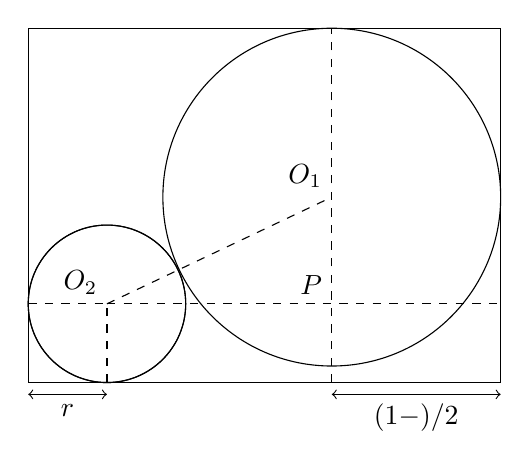
\begin{tikzpicture}[scale=0.5]
		\coordinate (a) at (0,0);
		\coordinate (b) at (12,0);
		\coordinate (c) at (0,9);
		\coordinate (d) at (12,9);
		\coordinate (e) at (2,0);
		\coordinate (f) at (12-4.29,0);
		\draw (0,0) rectangle (12,9);
		\draw (2,2) circle (2cm);
		x=4;
		\draw (12-4.29,9-4.29) circle (4.29 cm);
		\draw[dashed] (2,2) -- (12,2);
		\draw [dashed] (12-4.29,0) -- (12-4.29,9);
		\draw [dashed] (2,2) -- (12-4.29,9-4.29);
		\draw [dashed] (2,0) -- (2,2);
		\draw [dashed] (0,2) -- (2,2);
		\draw (2,2) circle (2cm);
		\node[above left] at (2,2) {$O_2$};
		\node[above left] at (12-4.29,9-4.29) {$O_1$};
		\node[above left] at (12-4.29,2) {$P$};
		\draw[<->] ([yshift=-0.3cm]f) -- ([yshift=-0.3cm]b) node[midway, below]{$(1-\eps)/2$};
		\draw[<->] ([yshift=-0.3cm]a) -- ([yshift=-0.3cm]e) node[midway, below]{$r$};
		\label{Figure 4}
		\end{tikzpicture}
		\caption{Worst case scenario for second biggest sphere in two dimensions.}
		\label{hypersphere}
	\end{figure}
	%\newpage
	% \\\includegraphics[width=10cm]{Images/hypersphere.jpeg}
	
	Let a huge circle of the minimum diameter $1-\eps$ be pushed to the rightmost corner of the augmented box centered at $O_1$. We try and fit a circle of radius $r$ in the bottom-left corner of the box centered at $O_2$. We notice that in 2 dimensions, $O_1 O_2 P$ forms a right triangle. $O_2 P= 1+\eps - r - (1-\eps)/2$, $O_1 P = 1 - r - (1-\eps)/2$, and $O_1 O_2 = r + (1-\eps)/2$. Applying Pythagorean theorem in two dimensions, we get $r=\frac{3}{2} (1+\eps) - \sqrt(2+3\eps)$. In d-dimensions, this generalises to $r= \frac{1}{2}+\frac{1}{d-1}+\eps( \frac{1}{2} + \frac{2}{d-1}) -\sqrt{\frac{(1+\eps)^2}{(d-1)^2}+\frac{1-\eps^2}{d-1}}$ and we are done.
\end{proof}

\begin{restatable}{lemma}{uniqhugeaabs}
	\label{uniqhuge}
	For any $0 < \eps \leqslant 1/2d^2$ for all $d \geqslant 2$, there can be at most one hypersphere in $P$ with a diameter larger than $1-\eps$.
\end{restatable}
\begin{proof}
	We always get at most one \textit{huge} hypersphere if the radius calculated in the lemma \ref{nextrad} is always less than $(1-\eps)/2$. We show that such an $\eps>0$ can always exist regardless of $d$.
	\[\frac{1}{2}+\frac{1}{d-1}+\eps( \frac{1}{2} + \frac{2}{d-1}) -\sqrt{\frac{(1+\eps)^2}{(d-1)^2}+\frac{1-\eps^2}{d-1}} \leqslant (1-\eps)/2 \]
	Analytically solving the quadratic equation, it always holds for \[\eps \leqslant \frac{\sqrt{d^3+3d^2-4d+1}-d}{d^2+3d-1} \leqslant \frac{1}{2d^2}\] where the bound is always positive for all $d \geqslant 2$.
\end{proof}

\begin{restatable}{theorem}{apxtheoremabs}
	\label{3apx}
	There is a polynomial time $3$-approximation algorithm for the $\mathsf{d-CSK}$ problem.
\end{restatable}
\begin{proof}
	We show that for values of $\eps<1/2d^2$ as given in lemma \ref{uniqhuge} we can always partition the augmented bin packing $P$ into three separate packings into unit hypercube bins $B_1, B_2,$ and $B_3$. Let the unique huge hypersphere that intersects both $\ell$ and $\ell'$ be called $C_{huge}$ and remove $C_{huge}$ from all other types of hyperspheres in $P$ as defined earlier. If there is no \textit{huge} hypersphere, then ignore this step. Now note that the set of type 1, type 2, type 3, type 2', type 3', and $C_{huge}$ form a partition of the hyperspheres in $P$.  
	\\We first pack $B_1$ using the same structure as in $P$ with hyperspheres of type 3' and type 2'. This is possible as no hypersphere of type 2' can intersect $\ell$ and we can simply remove the $\eps$-slab to the right of $\ell'$ and we get our bin packing $B_1$. We then pack $B_3$ with hyperspheres of type 2, type 3, and type 1. We then pack the unique hypersphere $C_{huge}$ which has a diameter of at most 1 in a unit bin $B_2$. Note here that we needed to have at most one $C_{huge}$ as the bin width could have been more than 1 even though the huge hyperspheres themselves had a diameter less than 1. We then return the bin out of $B_1, B_2, B_3$ with the most profit.
	\\The running time of this algorithm is clearly polynomial as the we get the augmented packing from lemma \ref{extended-wowa} in polynomial time and the partitioning takes linear time. 
	 Since we return the bin with the maximum weight, we return a instance of $\mathsf{d-CSK}$ with a profit of at least $\frac{1}{3} w(\OPT)$. 
\end{proof}

\subsection{$(2+\eps)$-approximation algorithm for \(d\leq 8\)}
The main goal of this section is to show that the packings we return for bins $B_1$ and $B_3$ in the $3$-approximation algorithms can in fact be packed into a single bin for $d\leqslant 8$. When there are no \textit{huge} hyperspheres with a diameter greater than $(1-\eps)$, a simple argument for packing in two bins can be made. Also, from lemma \ref{uniqhuge} we know that for small enough values of $\eps$, there can be at most one \textit{huge} hypersphere.

\begin{restatable}{lemma}{nohugelemmaapx}
	\label{nohuge}
	If there are no \textit{huge} hyperspheres with a diameter bigger than $1-\eps$, then the augmented bin packing $P$ can be partitioned into two unit bin packings $B_1$ and $B_2$.
\end{restatable}
\begin{proof}
	We partition using the same algorithm as in theorem \ref{3apx} into three unit bins. However the bin that contained the \textit{huge} hypersphere before is now completely empty, so we simply return the other two bins.
\end{proof}

If we have a unique \textit{huge} hypersphere $C_{huge}$, we again show that we can pack $P$ into two different unit bin packings $B_1$ and $B_2$. Let us define another $\eps$-slab $D$ which is parallel to $\ell$ and $\ell'$ and is situated exactly halfway between the two and has $\eps$-width. To use our strategy we need an "empty" $\eps$-slab $S$ in the middle of the augmented bin, which restricts the dimension to $d\leqslant 8$.

\begin{figure}[ht]
	\begin{center}
		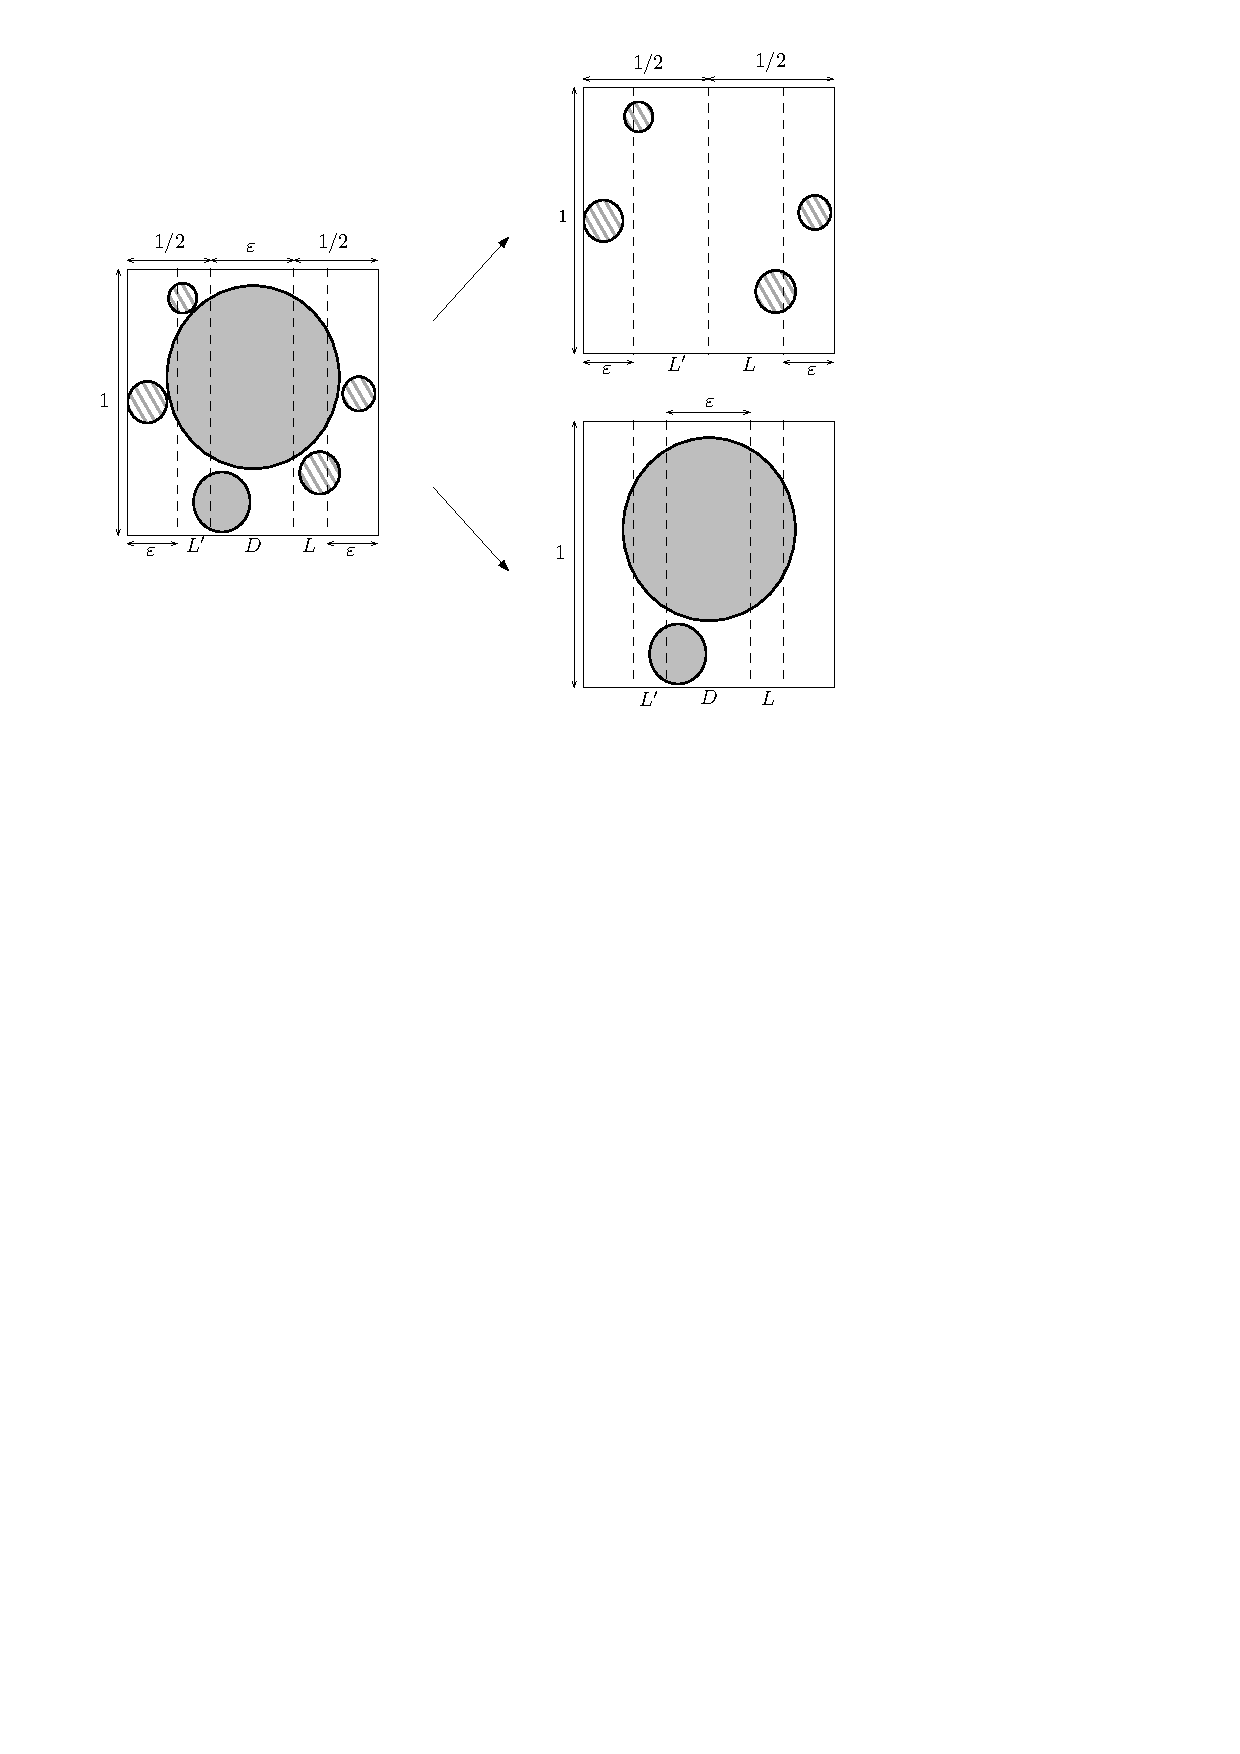
\includegraphics[width=10cm]{Figures/hypersphere_bin_generation.pdf}
		\caption{Dividing augmented packing $P$ into two unit bin packings $B_1$ and $B_2$ with the help of $\eps$-slab $D$}
		\label{fig:partition-img-2}
	\end{center}
	
\end{figure}

\begin{restatable}{lemma}{mindistlemma}
	\label{mindist}
	For $\eps < 1/d^2.2^d$ and $d \leqslant 8$, the distance between any arbitrary type 2 hypersphere and any arbitrary hypersphere of type 2' is at least $\eps$.
\end{restatable}
\begin{proof}
	If the diameter of the hypersphere calculated in lemma \ref{nextrad} is smaller than $1/2 - \eps$, this is true as the distance between $\ell$ and $D$, $\ell'$ and $D$ is $1/2 - \eps$.   
	\[\frac{1}{2}+\frac{1}{d-1}+\eps( \frac{1}{2} + \frac{2}{d-1}) -\sqrt{\frac{(1+\eps)^2}{(d-1)^2}+\frac{1-\eps^2}{d-1}} \leq 1/4 - \frac{\eps}{2}\]
	This inequality holds true for some positive value of $\eps$ only for $d\leq 8$.  
\end{proof}

\begin{restatable}{theorem}{approxtheorem}
	There is a polynomial time $(2+\eps)$-approximation algorithm for $\mathsf{d-CSK}$ for dimension $d<8$ and $0<\eps<1/4d^2.5^{2d+3}$.
\end{restatable}
\begin{proof}
	We choose $\eps$ small enough from lemma \ref{uniqhuge} such that there can be at most one \textit{huge} hypersphere of diameter bigger than $1-\eps$. Now, if there are no hyperspheres in the augmented packing $P$ obtained from lemma \ref{extended-wowa} with a diameter bigger than $1-\eps$, we proceed to partition and pack $P$ into two augmented unit bins $B_1$ and $B_2$ using lemma \ref{nohuge}. 
	\\In the case where there is a unique \textit{huge} hypersphere, we choose $\eps$ small enough from lemma \ref{uniqhuge} such that type 2 and type 2' hyperspheres in $P$ leave an empty $\eps$-strip $D$ between them in the middle of the augmented bin. Now we pack the only huge hypersphere $C_{huge}$ and type 1 hyperspheres into $B_2$. We now can simply remove the strip $D$ and join the segments to get a unit bin packing $B_1$ of hyperspheres of types 2,3,2',3'.
	\\At the end we return packing out of $B_1,B_2$ with maximum weight. This algorithm is clearly polynomial as we get the augmented packing from lemma \ref{extended-wowa} in polynomial time and the partitioning takes linear time. The algorithm returns an instance of $\mathsf{d-CSK}$ of total weight at least of $\frac{(1-\eps)}{2}w(\OPT)$.
\end{proof}